\bigskip

\item Which of the following could describe the graph below?

% \resizebox{3in}{!}{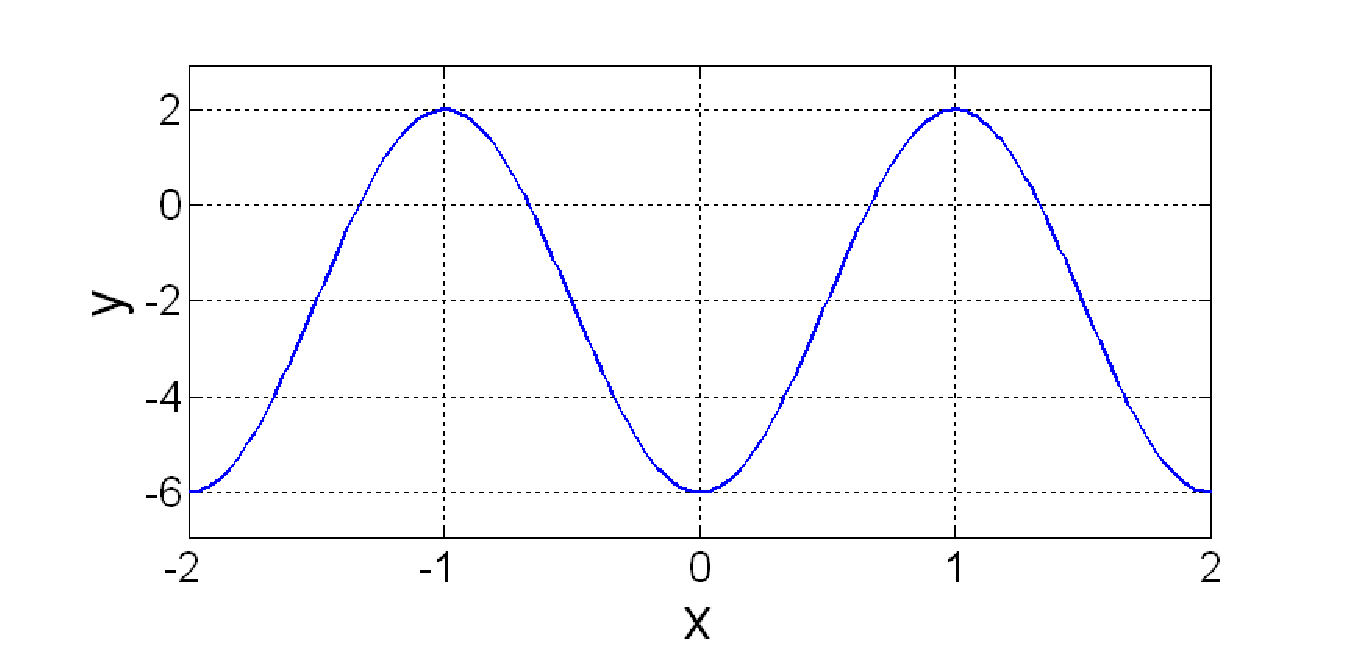
\includegraphics{SVC.01.05.050.ps}}

\begin{minipage}{0.4\columnwidth}
    \begin{enumerate}
        \item $y = 4 \sin\left( \pi x - \frac{\pi}{2}\right) - 2$
        \item $y = -4 \sin\left( \pi x + \frac{\pi}{2}\right) - 2$
        \item $y = -4 \cos( \pi x ) - 2$
        \item $y = 4 \cos( \pi ( x+1) ) - 2$
        \item All of the above
        \item More than one, but not all of the above
    \end{enumerate}
\end{minipage}
\begin{minipage}{0.6\columnwidth}
    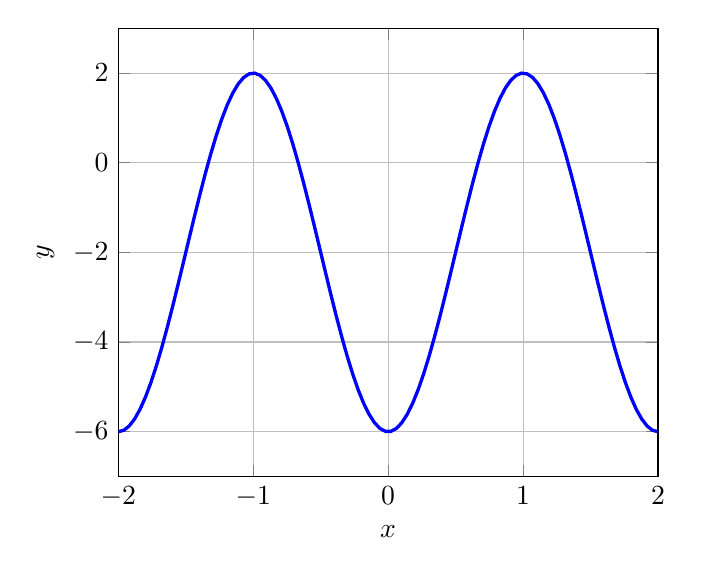
\begin{tikzpicture}
        \begin{axis}[xlabel={$x$}, ylabel={$y$}, xmin=-2, xmax=2,
                ymin=-7, ymax=3, grid]
                \addplot[color=blue, very thick,domain=-2:2, samples=100]
                {-4*cos(pi*deg(x))-2};
            \end{axis}
    \end{tikzpicture}
\end{minipage}

% by Carroll College MathQuest
